\section{سوال اول}
 در این بخش از مدل ارائه شده در تمرین سوم استفاده شده است، بنابراین از توضیح مجدد آن خودداری شده است. البته مدل جهت استفاده بهتر برای هدایت دو نقطه‌ای اندکی تغیر کرده است که در ادامه به توضیح آن پرداخته خواهد شد.

\subsection{بخش الف}
این بخش شامل دو قسمت بررسی شرایط اولیه و بررسی هدایت دو نقطه‌ای است.
\subsubsection{مسیر برخورد}
در این قسمت با استفاده از بهینه‌سازی (کد \lr{optimization.m}) زوایای اولیه جهت قرارگیری موشک بر روی مسیر برخورد\LTRfootnote{Collision Course}
قرار گیرد. شرایط اولیه و فاصله ازدست‌دهی در جدول \ref{Q1_part_a_sec_I} آورده شده است.

\begin{table}[H]
	\caption{شرایط اولیه و فاصله ازدست‌دهی }
	\label{Q1_part_a_sec_I}
	\centering
	\begin{tabular}{cc}
		\hline
		Value &  Parameter \\
		\hline
		\lr{\ang{72.1561}} & \lr{$\theta_0$}\\
		\lr{\ang{16.4500}}  & $\psi_0$ \\ 
		\lr{0.3738}& \lr{Miss Distance (m)}  \\
		\hline
	\end{tabular}
\end{table}

\begin{figure}[H]
	\centering
	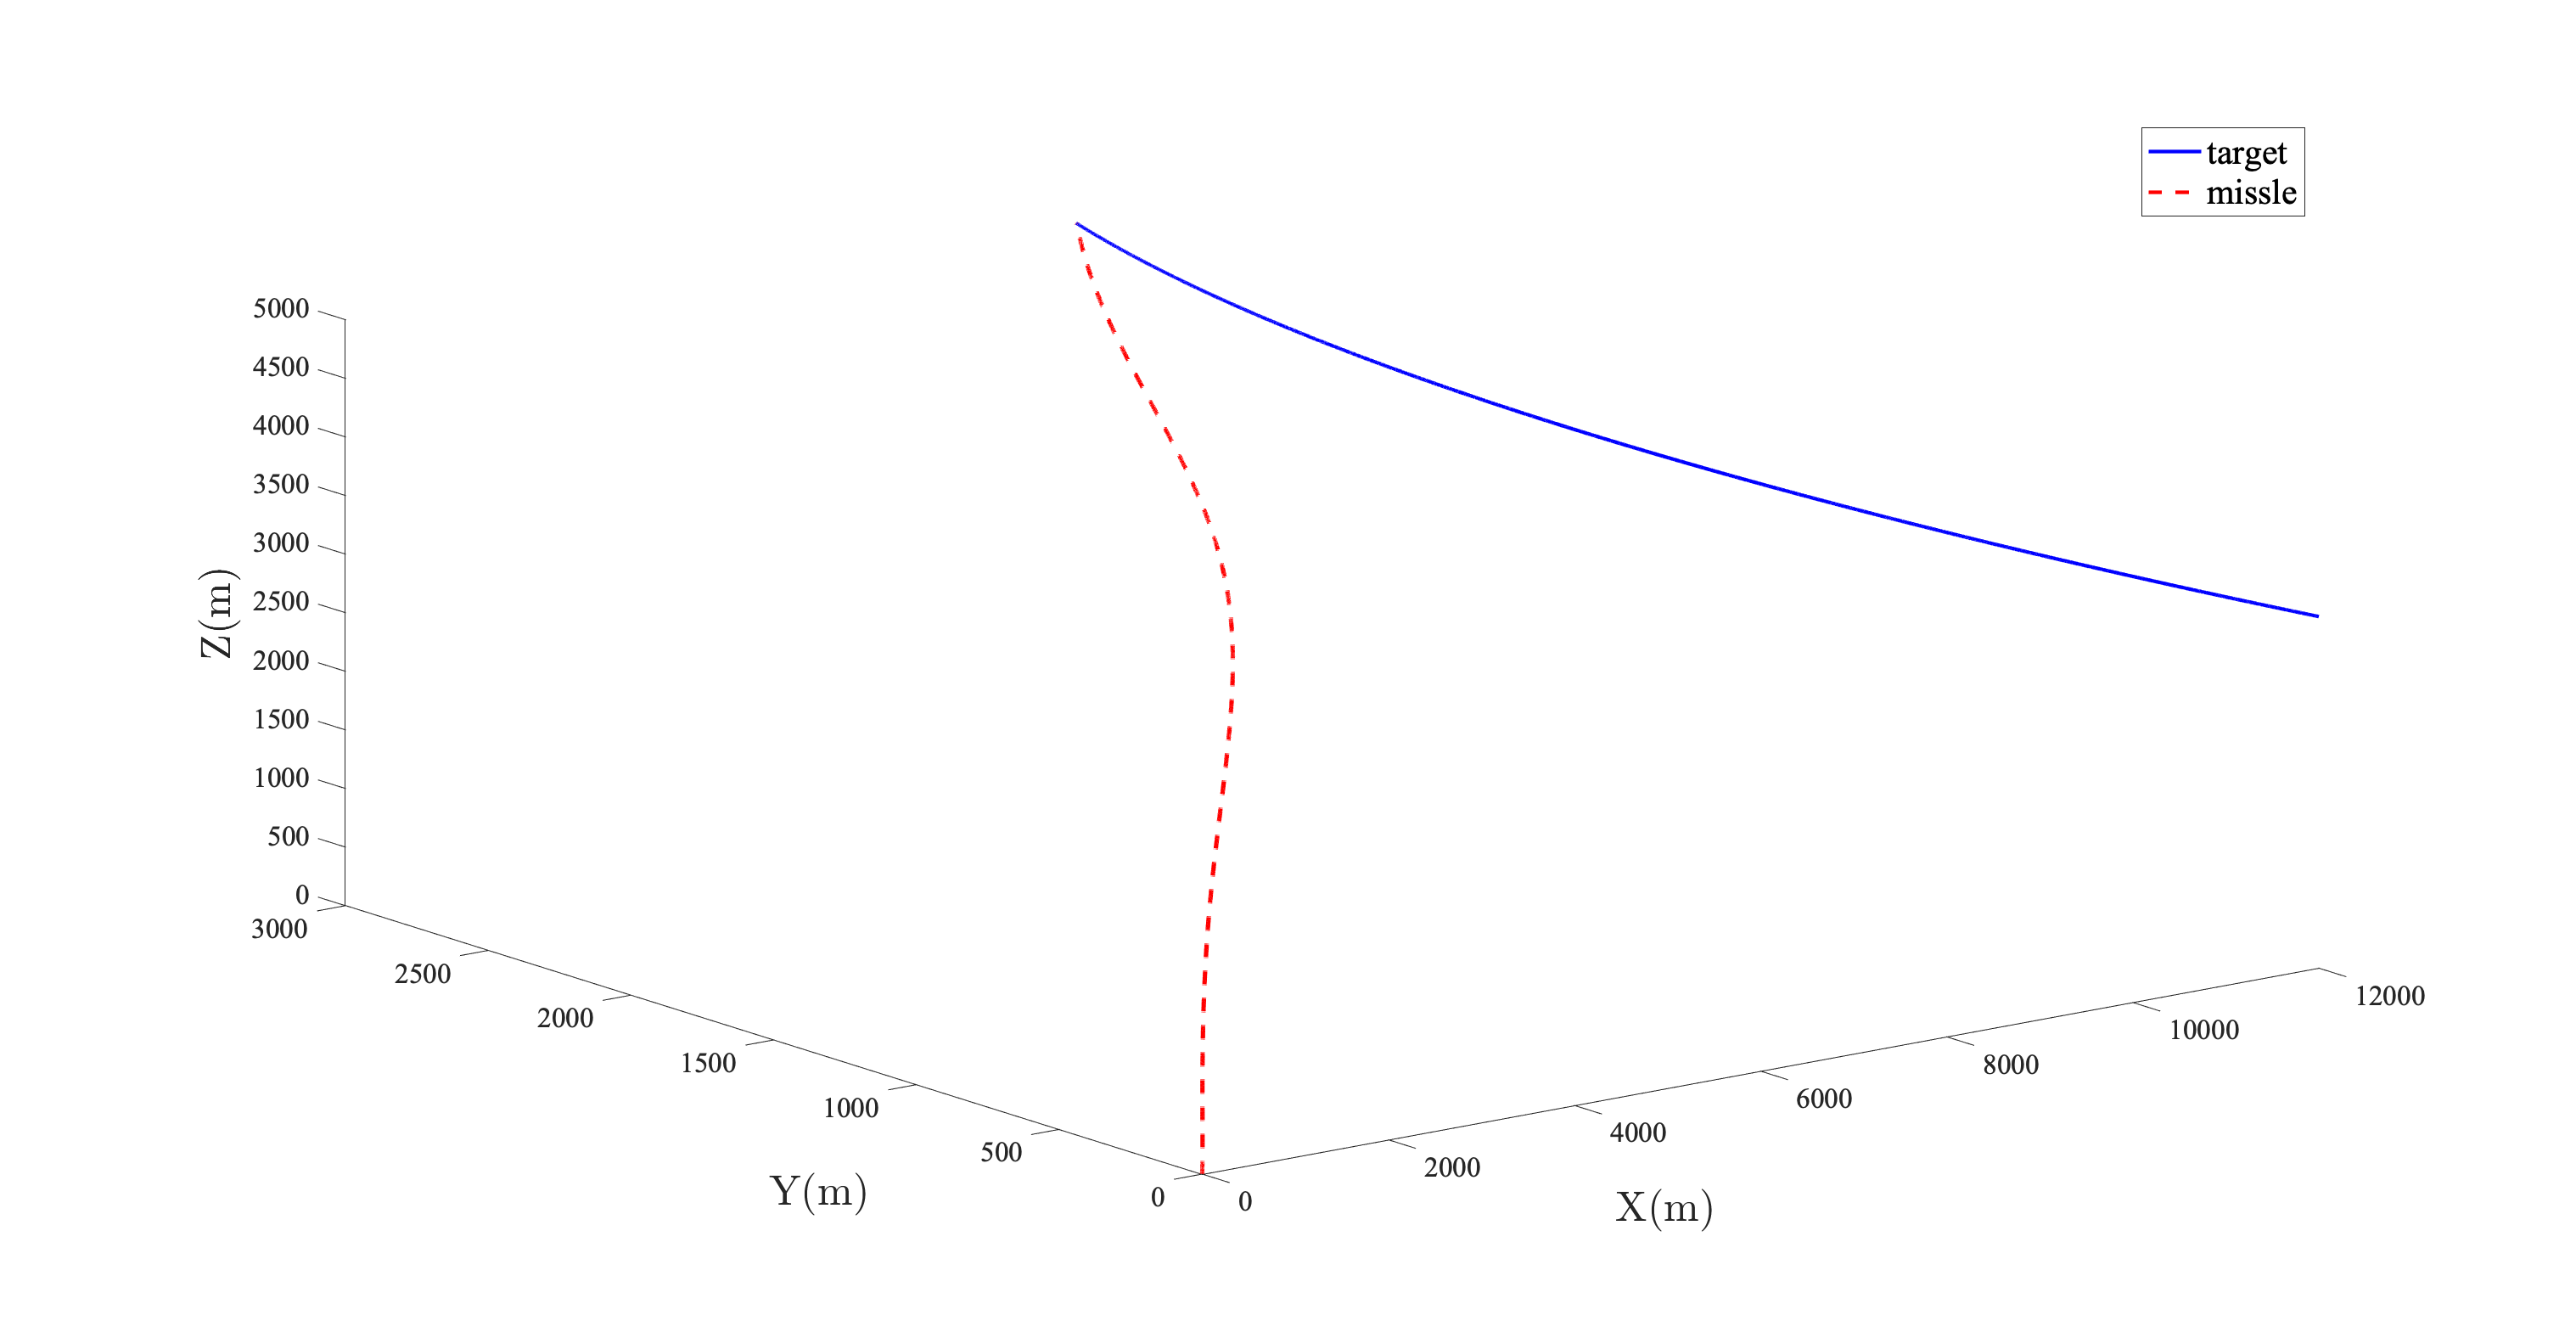
\includegraphics[width=\linewidth]{../Figure/Q1/a/collision_course}
	\caption{موقعیت موشک و هدف به صورت سه بعدی با شرایط اولیه مسیر برخورد}
\end{figure}

\begin{figure}[H]
	\centering
	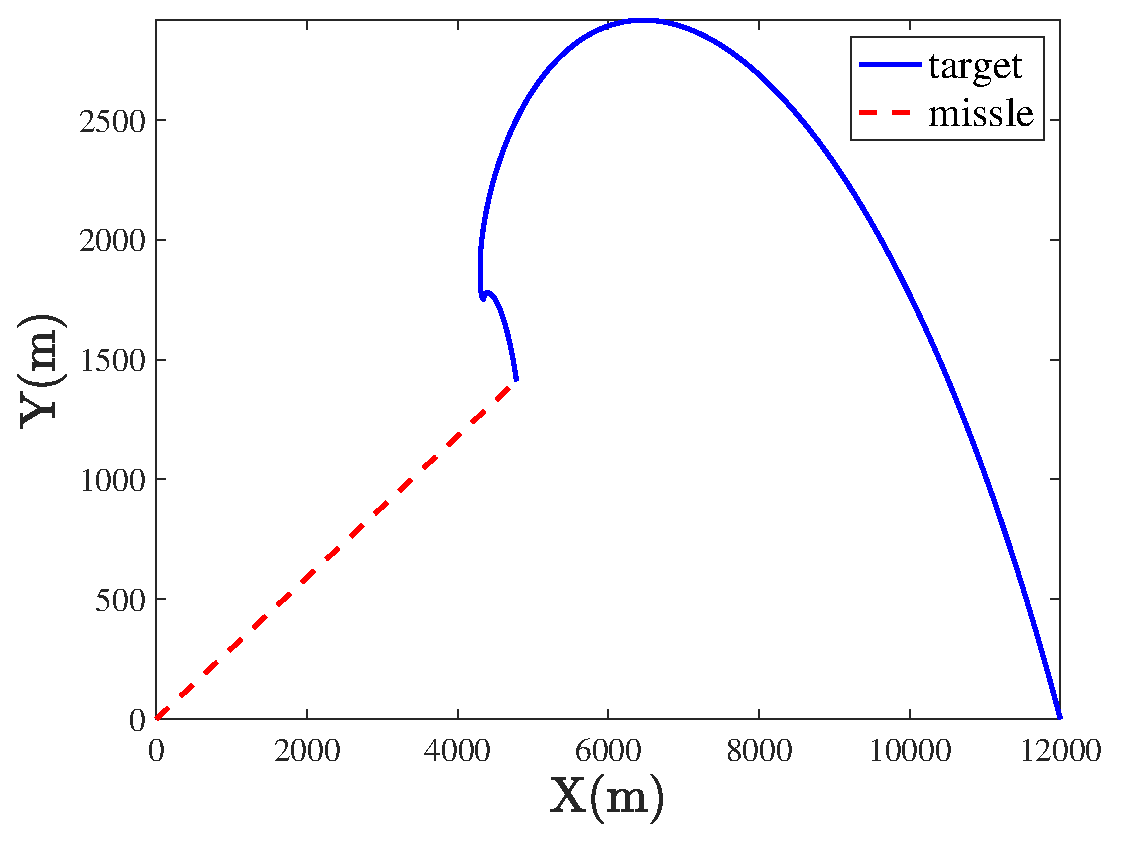
\includegraphics[width=.75\linewidth]{../Figure/Q1/a/xy_sec_I}
	\caption{موقعیت موشک و هدف در صفحه \lr{xy}
		با شرایط اولیه مسیر برخورد}
\end{figure}

\begin{figure}[H]
	\centering
	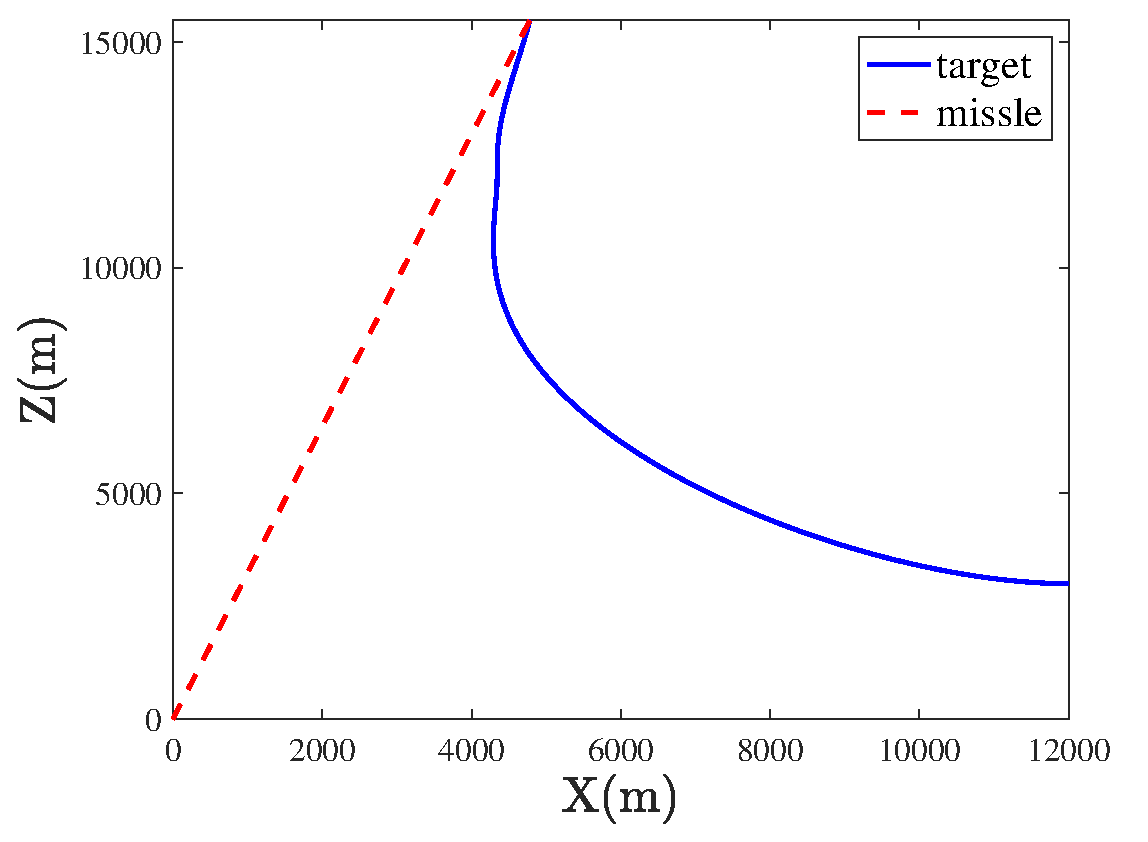
\includegraphics[width=.75\linewidth]{../Figure/Q1/a/xz_sec_I}
	\caption{موقعیت موشک و هدف در صفحه \lr{xz}
		با شرایط اولیه مسیر برخورد}
\end{figure}

\begin{figure}[H]
	\centering
	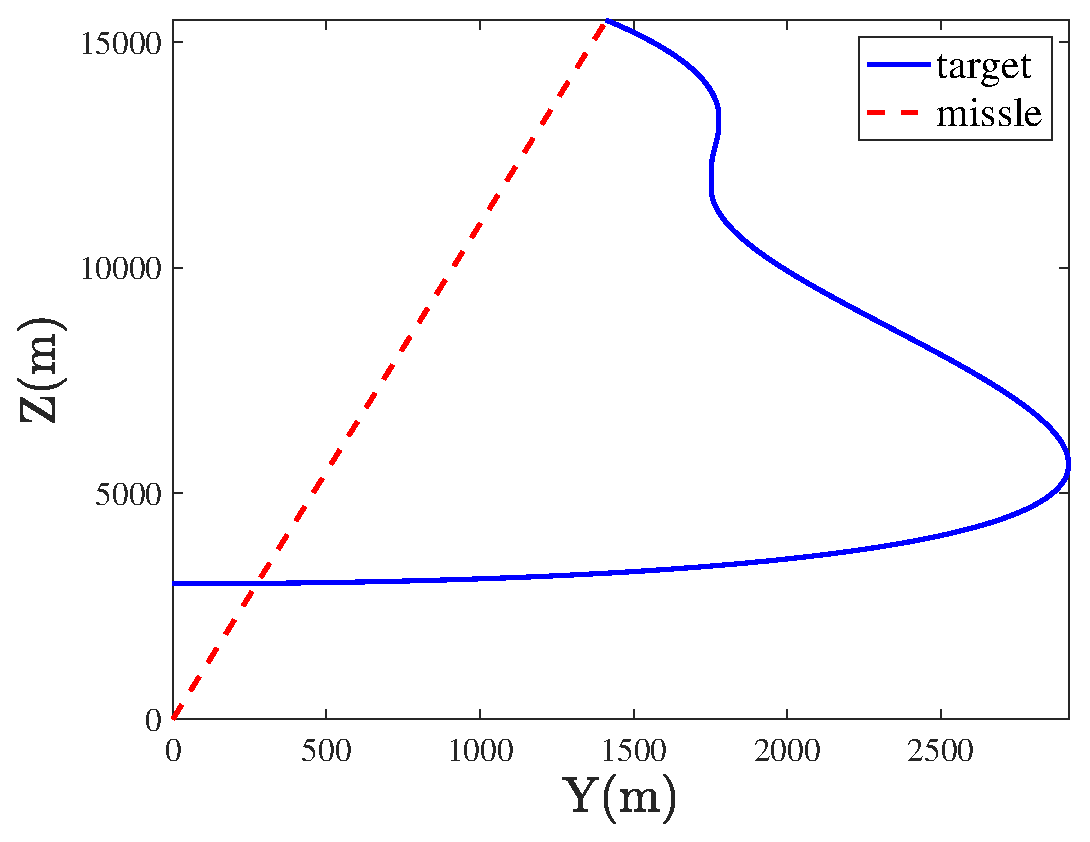
\includegraphics[width=.75\linewidth]{../Figure/Q1/a/yz_sec_I}
	\caption{موقعیت موشک و هدف در صفحه \lr{yz}
		با شرایط اولیه مسیر برخورد}
\end{figure}


\subsubsection{هدایت دو نقطه‌ای}

در این بخش به بررسی هدایت تناسبی پرداخته شده است. نتایج برای
$N=4$
در ادامه آورده شده است.

\begin{table}[H]
	\caption{پارامترها و نتایج هدایت تناسبی}
	\centering
	\begin{tabular}{cc}
		\hline
		Value &  Parameter \\
		\hline
		\lr{4} & \lr{$N$}\\
		\lr{\ang{72.1561}} & \lr{$\theta_0$}\\
		\lr{\ang{16.4500}}  & $\psi_0$ \\ 
		\lr{0.8344}& \lr{Miss Distance (m)}  \\
		\lr{1278}& \lr{Control effort}  \\
		\hline
	\end{tabular}
\end{table}



\begin{figure}[H]
	\centering
	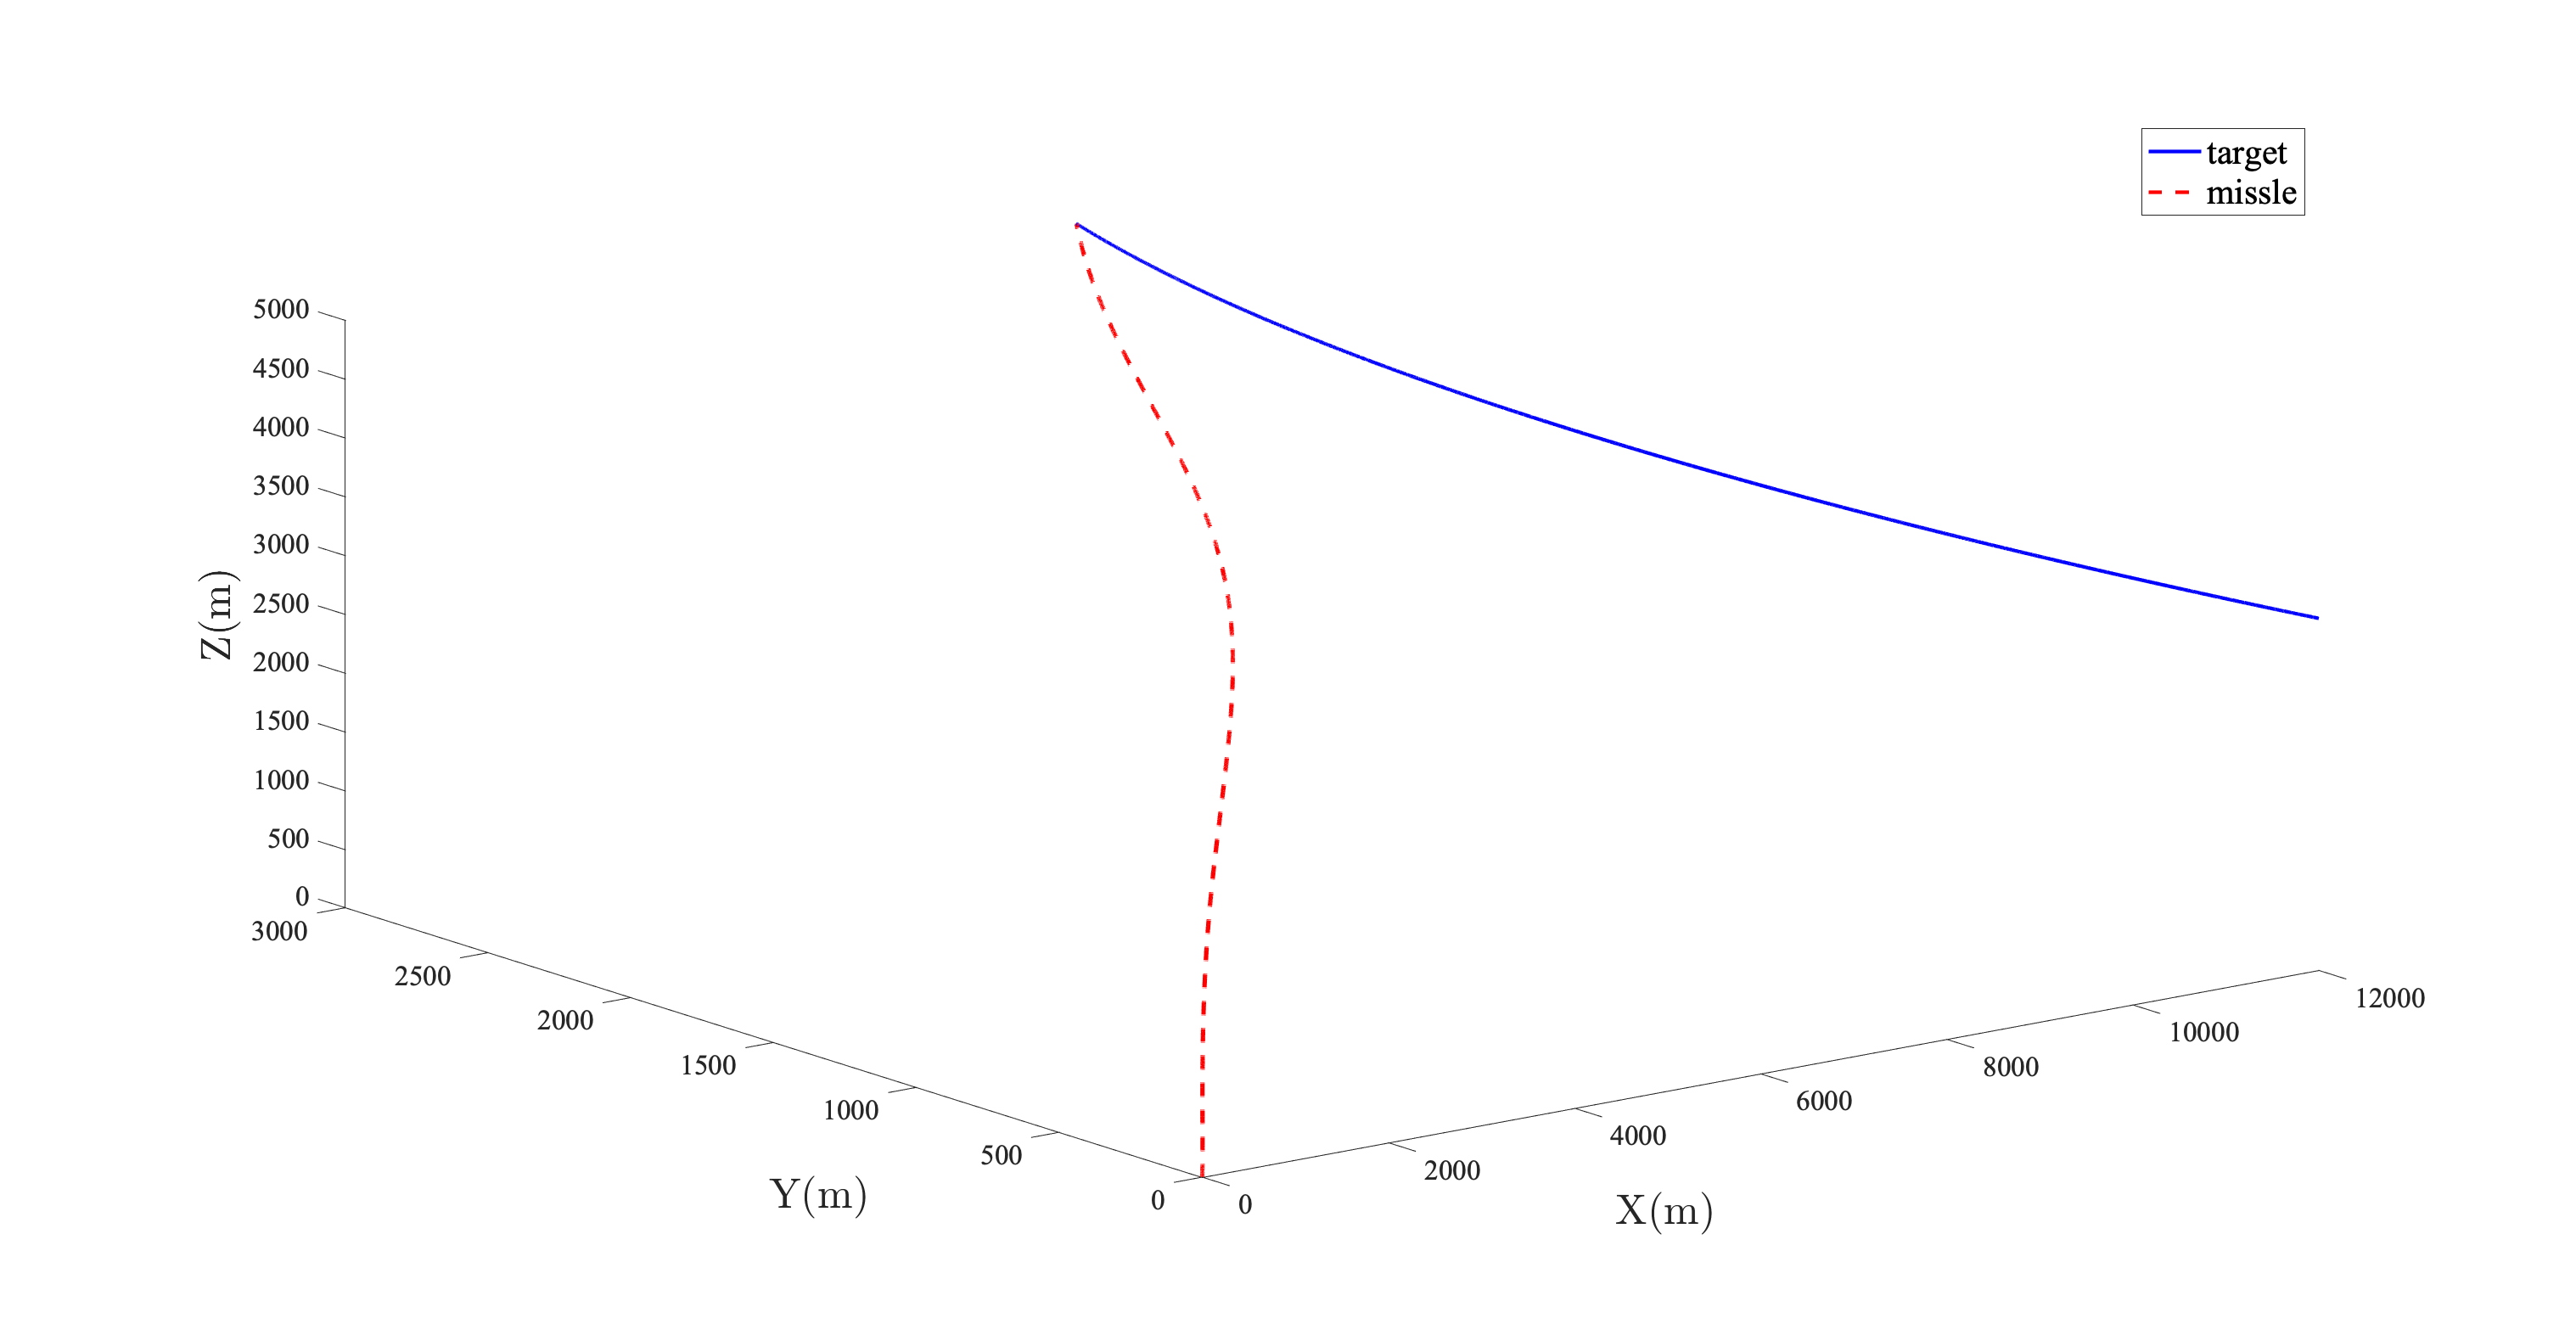
\includegraphics[width=\linewidth]{../Figure/Q1/a/two_point}
	\caption{موقعیت موشک و هدف به صورت سه بعدی با شرایط اولیه مسیر برخورد در هدایت تناسبی}
\end{figure}

\begin{figure}[H]
	\centering
	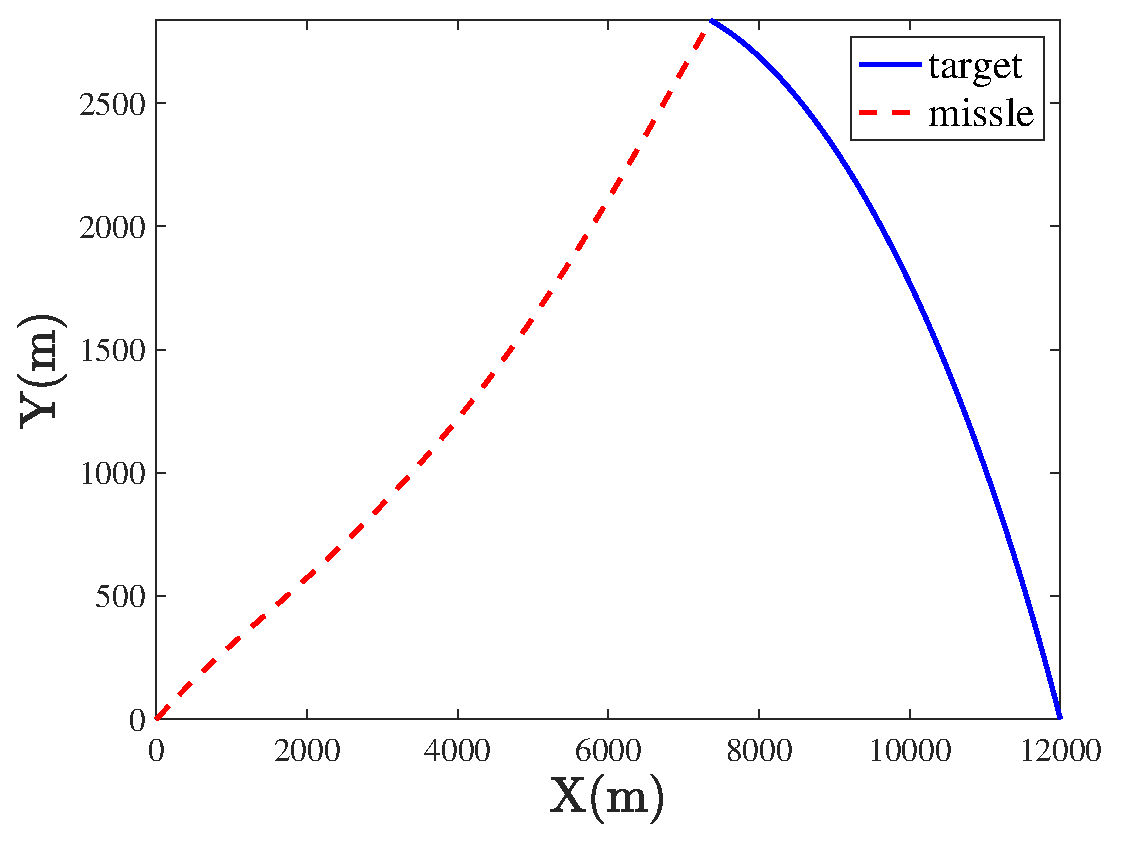
\includegraphics[width=.75\linewidth]{../Figure/Q1/a/xy_sec_II}
	\caption{موقعیت موشک و هدف در صفحه \lr{xy}
		با شرایط اولیه مسیر برخورد در هدایت تناسبی}
\end{figure}

\begin{figure}[H]
	\centering
	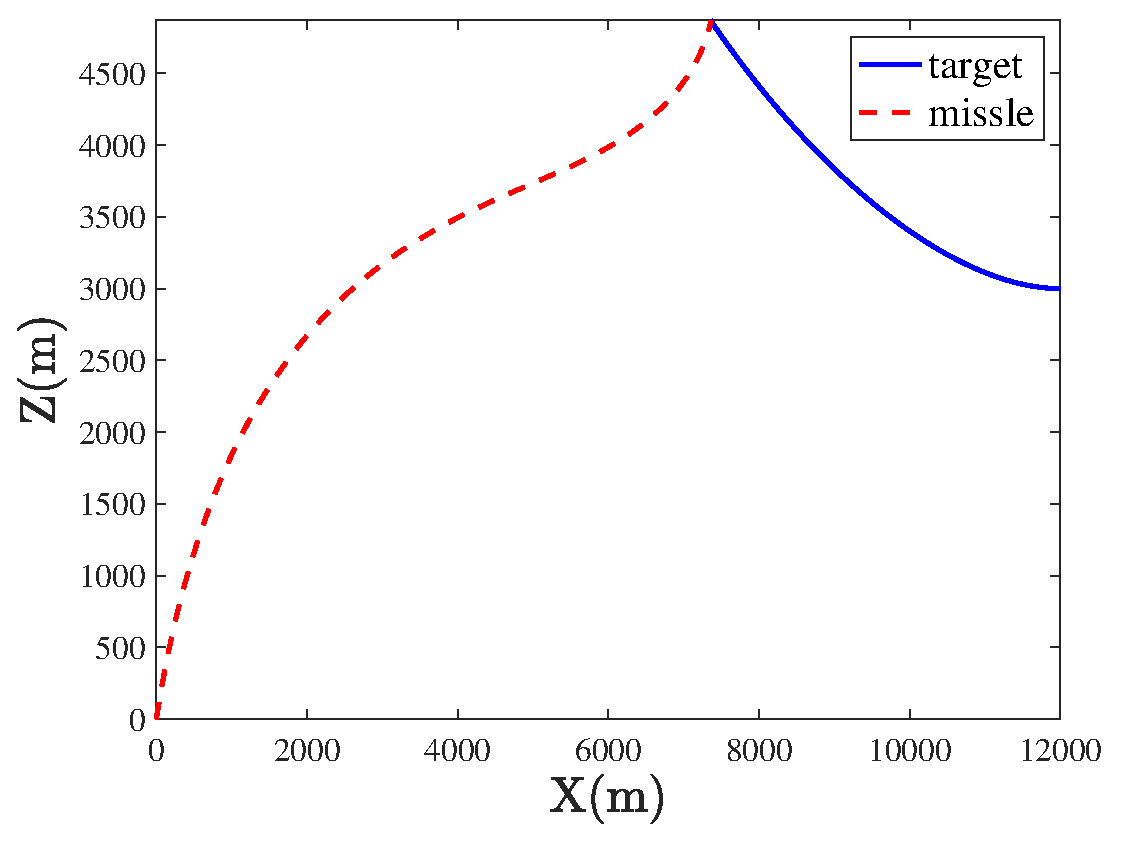
\includegraphics[width=.75\linewidth]{../Figure/Q1/a/xz_sec_II}
	\caption{موقعیت موشک و هدف در صفحه \lr{xz}
		با شرایط اولیه مسیر برخورد در هدایت تناسبی}
\end{figure}

\begin{figure}[H]
	\centering
	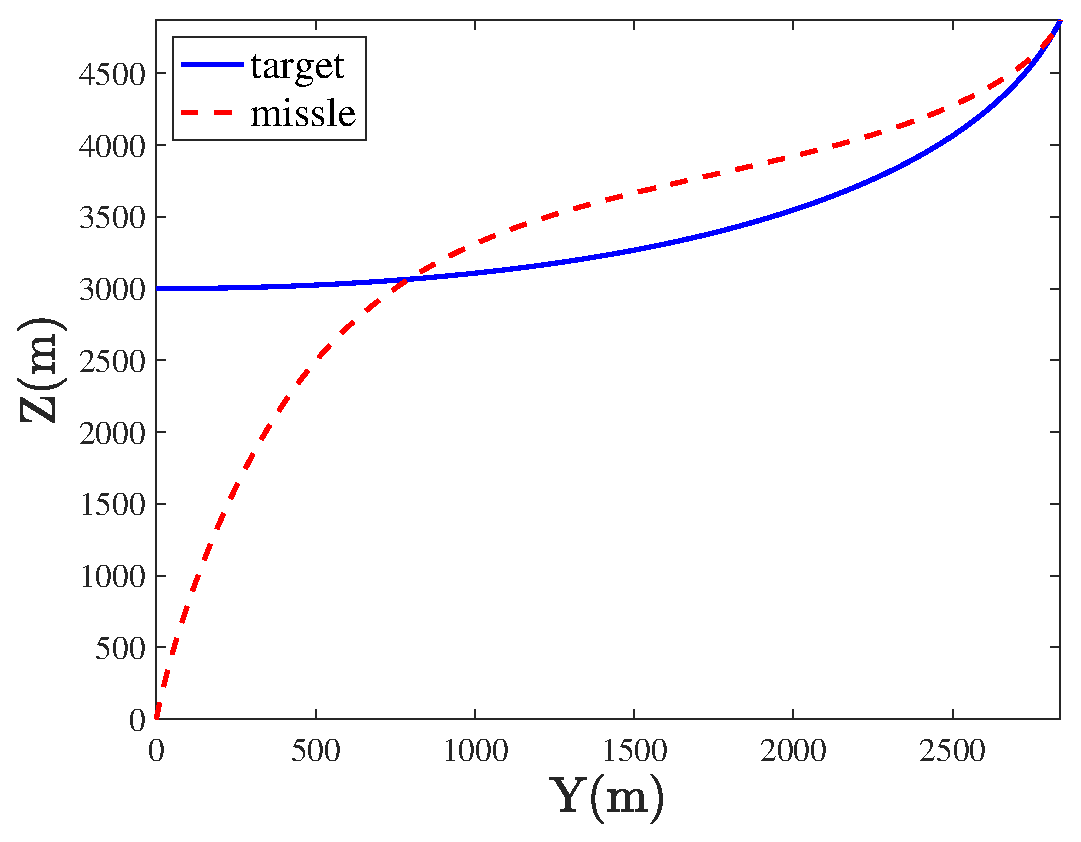
\includegraphics[width=.75\linewidth]{../Figure/Q1/a/yz_sec_II}
	\caption{موقعیت موشک و هدف در صفحه \lr{yz}
		با شرایط اولیه مسیر برخورد در هدایت تناسبی}
\end{figure}



\begin{figure}[H]
	\centering
	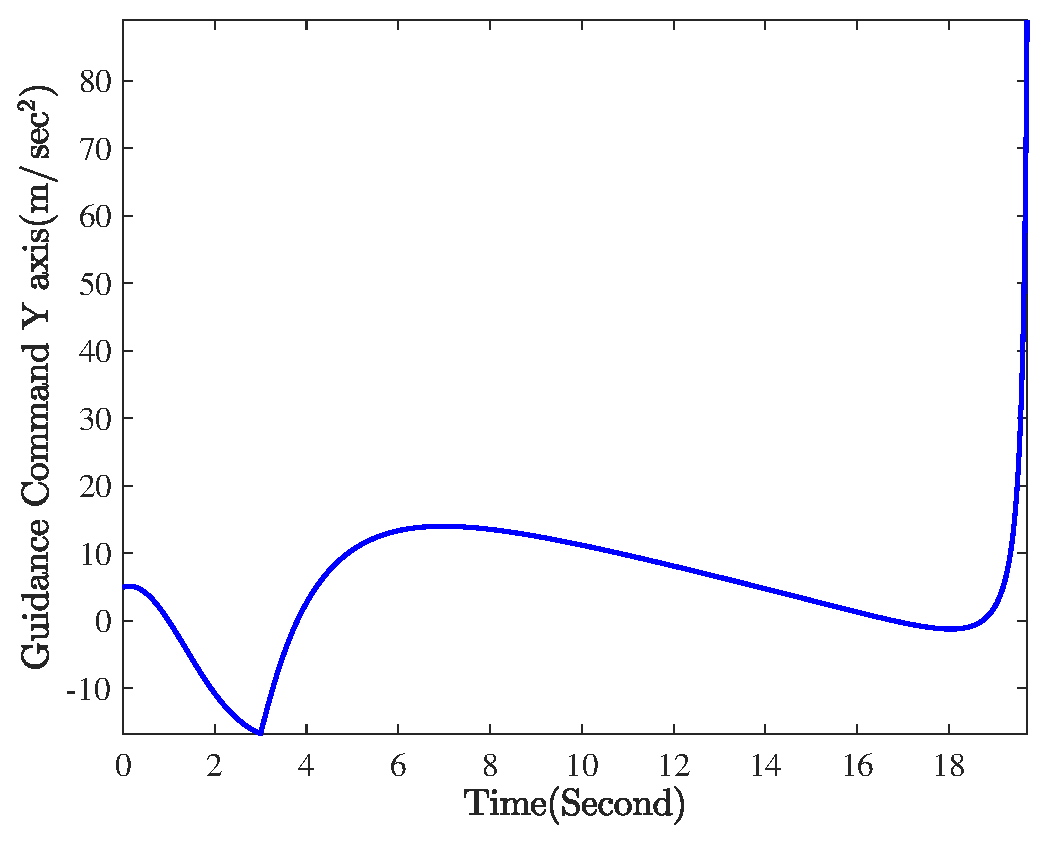
\includegraphics[width=.75\linewidth]{../Figure/Q1/a/GC_y}
	\caption{فرمان هدایت تناسبی در جهت محور \lr{y}}
\end{figure}

\begin{figure}[H]
	\centering
	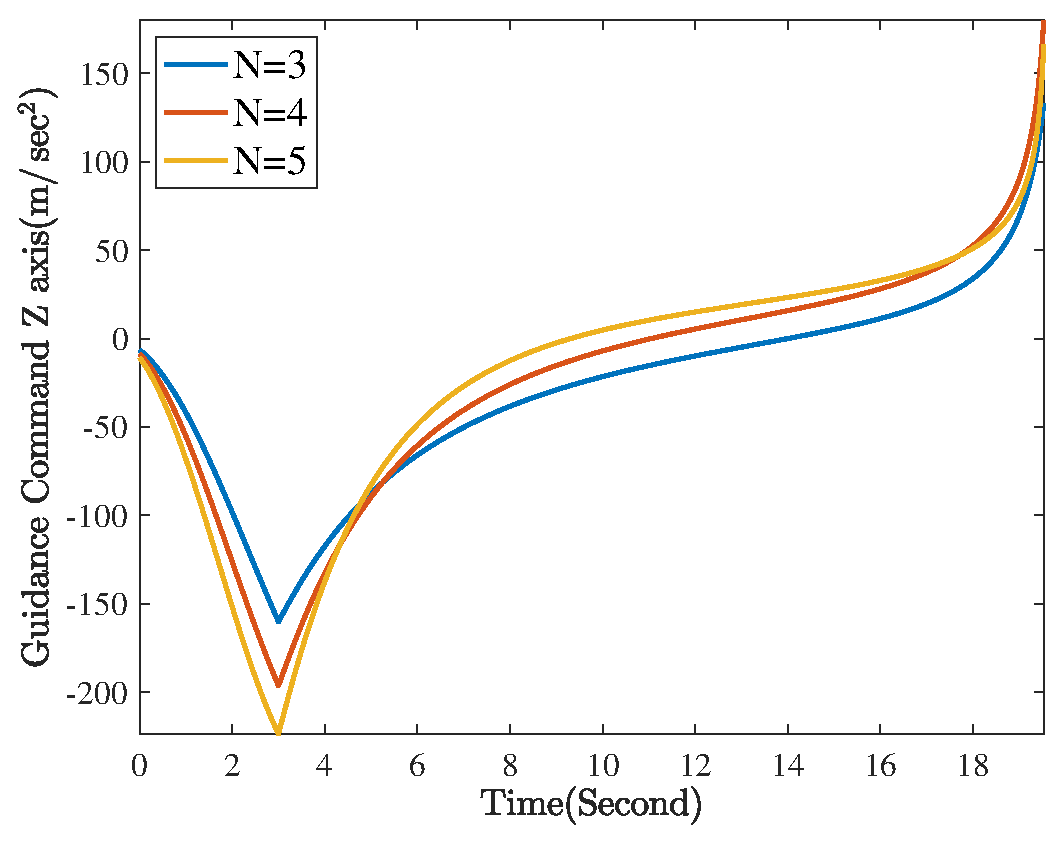
\includegraphics[width=.75\linewidth]{../Figure/Q1/a/GC_z}
	\caption{فرمان هدایت تناسبی در جهت محور \lr{z}}
\end{figure}

\begin{figure}[H]
	\centering
	\includegraphics[width=.75\linewidth]{../Figure/Q1/a/CC_y}
	\caption{فرمان کنترل‌کننده در جهت محور \lr{y}}
\end{figure}

\begin{figure}[H]
	\centering
	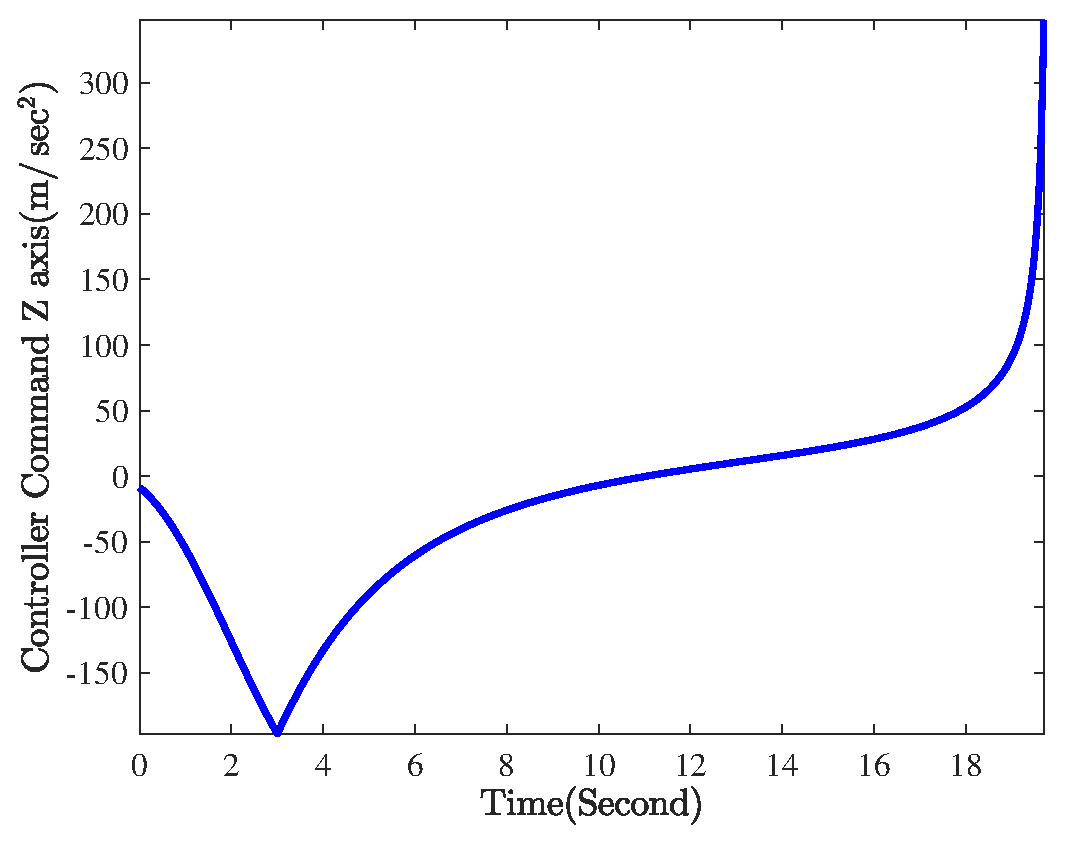
\includegraphics[width=.75\linewidth]{../Figure/Q1/a/CC_z}
	\caption{فرمان کنترل‌کننده در جهت محور \lr{z}}
\end{figure}

یرخ چرخش خط دید حکل محکر z y ادی

\begin{figure}[H]
	\centering
	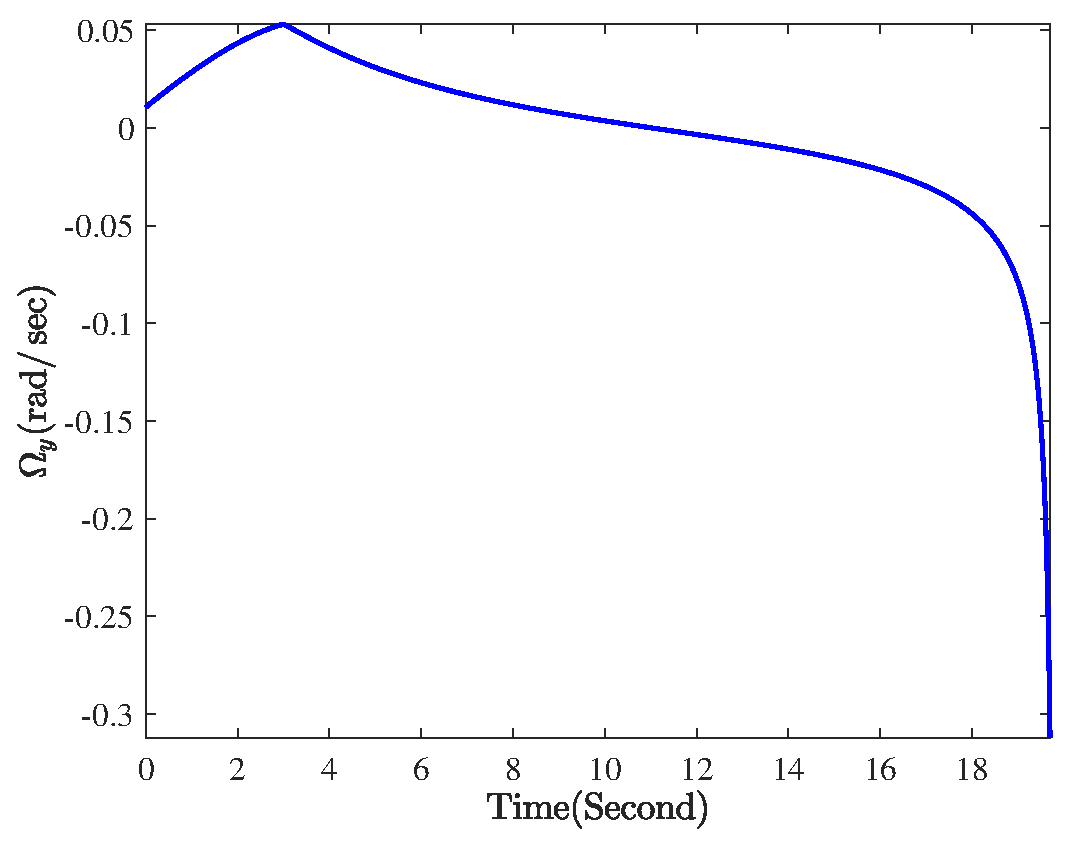
\includegraphics[width=.75\linewidth]{../Figure/Q1/a/Omega_y}
	\caption{نرخ چرخش خط دید حول محور \lr{y}}
\end{figure}

\begin{figure}[H]
	\centering
	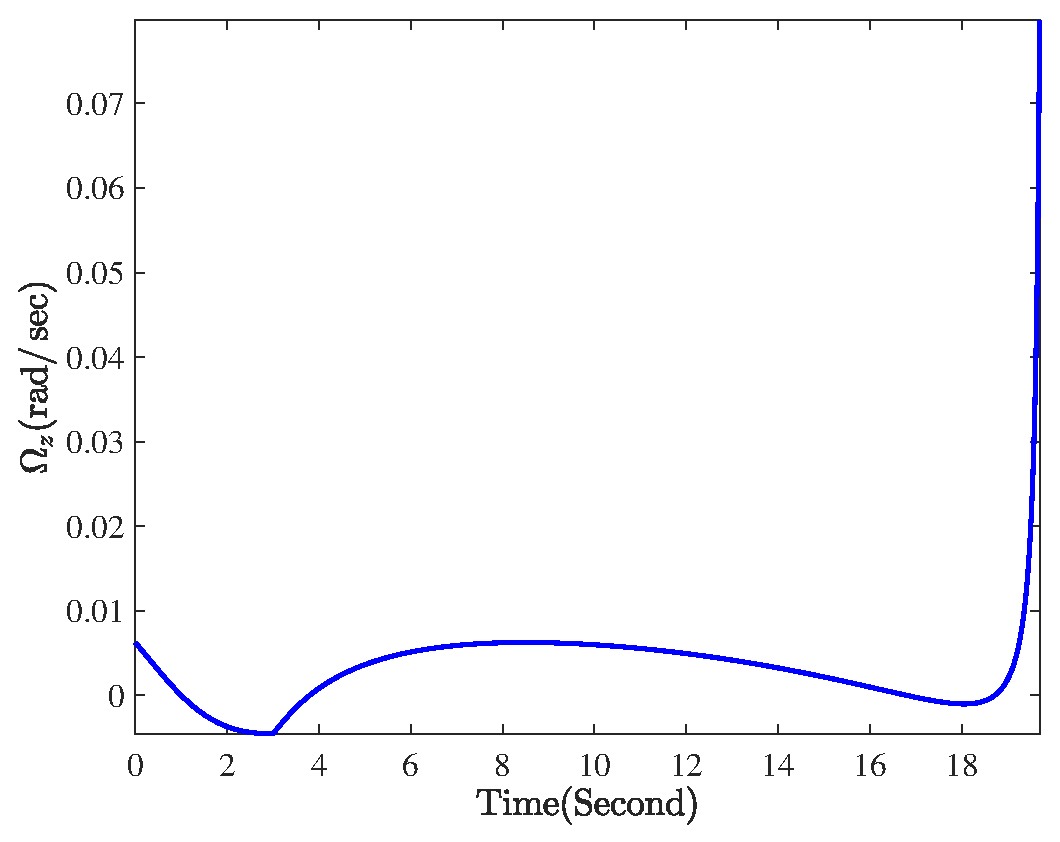
\includegraphics[width=.75\linewidth]{../Figure/Q1/a/Omega_z}
	\caption{نرخ چرخش خط دید حول محور \lr{z}}
\end{figure}
